\section{Sequence of Component/Function Integration}
\label{sec:sequence-integration}

\subsection{Software Integration Sequence}
The integration sequence of the components is described in~\autoref{tab:components-integration} and in~\autoref{fig:components-integration}.

The components are tested from the most independent to the less one. This gives the opportunity to avoid the implementation of useless stubs, because, when less independent components are tested, the components which they rely on have already been integrated.
The components are integrated within their classes in order to create an integrated subsystem which is ready to subsystem integration.

\begin{table}
    \centering
    \begin{tabular}{| l | l | l | l |}
    	\hline
	N. & Subsystem & Component & Integrates with \\
	\hline
	1 & Database, Business & (JEB) TaxiLog & DBMS\\
	2 & Database, Business & (JEB)  Ride & DBMS\\
	3 & Database, Business & (JEB) User & DBMS\\
	4 & Database, Business & (JEB) Passenger & DBMS\\
	5 & Database, Business & (JEB) TaxiDriver & DBMS\\
	6 & Business & (SB) TaxiManager & TaxiQueueManager, TaxiDriver\\
	7 & Business & (SB) RideManager & HistoryManager, User, Passenger, TaxiLog, Ride\\
	8 & Business & (SB) RideManager & ReservedRidePlugin\\
	9 & Business & (SB) RideManager & SharedRidePlugin\\
	10  & Business & (SB) UserManager & EmailSender, User\\
	11  & Business & (EJB container) TaxiManagerContainer & TaxiManager\\
	12  & Business & (EJB container) RideManagerContainer & RideManager, HistoryManager\\
	13  & Business & (EJB container) UserManagerContainer & UserManager, EmailSender\\
	14  & Business & Controller & TaxiManagerContainer, RideManagerContainer, UserManagerContainer, ConfiguratorBean\\
	15  & Mobile & UIManager & UIKit\\
	16  & Mobile & UIManager & android.view\\
	17  & Mobile & GPSManager & CoreLocation\\
	18  & Mobile & GPSManager & LocationListener\\
	19  & Mobile & Controller & UIManager, GPSManager, ResourceLoader\\
	20  & Web & WebController & JavaServerFaces\\
	21 & Web & WebContainer & WebController\\
	\hline
    \end{tabular}
    \caption{Integration of the system component.}
    \label{tab:components-integration}
\end{table}

\begin{figure}[h]
    \centering
    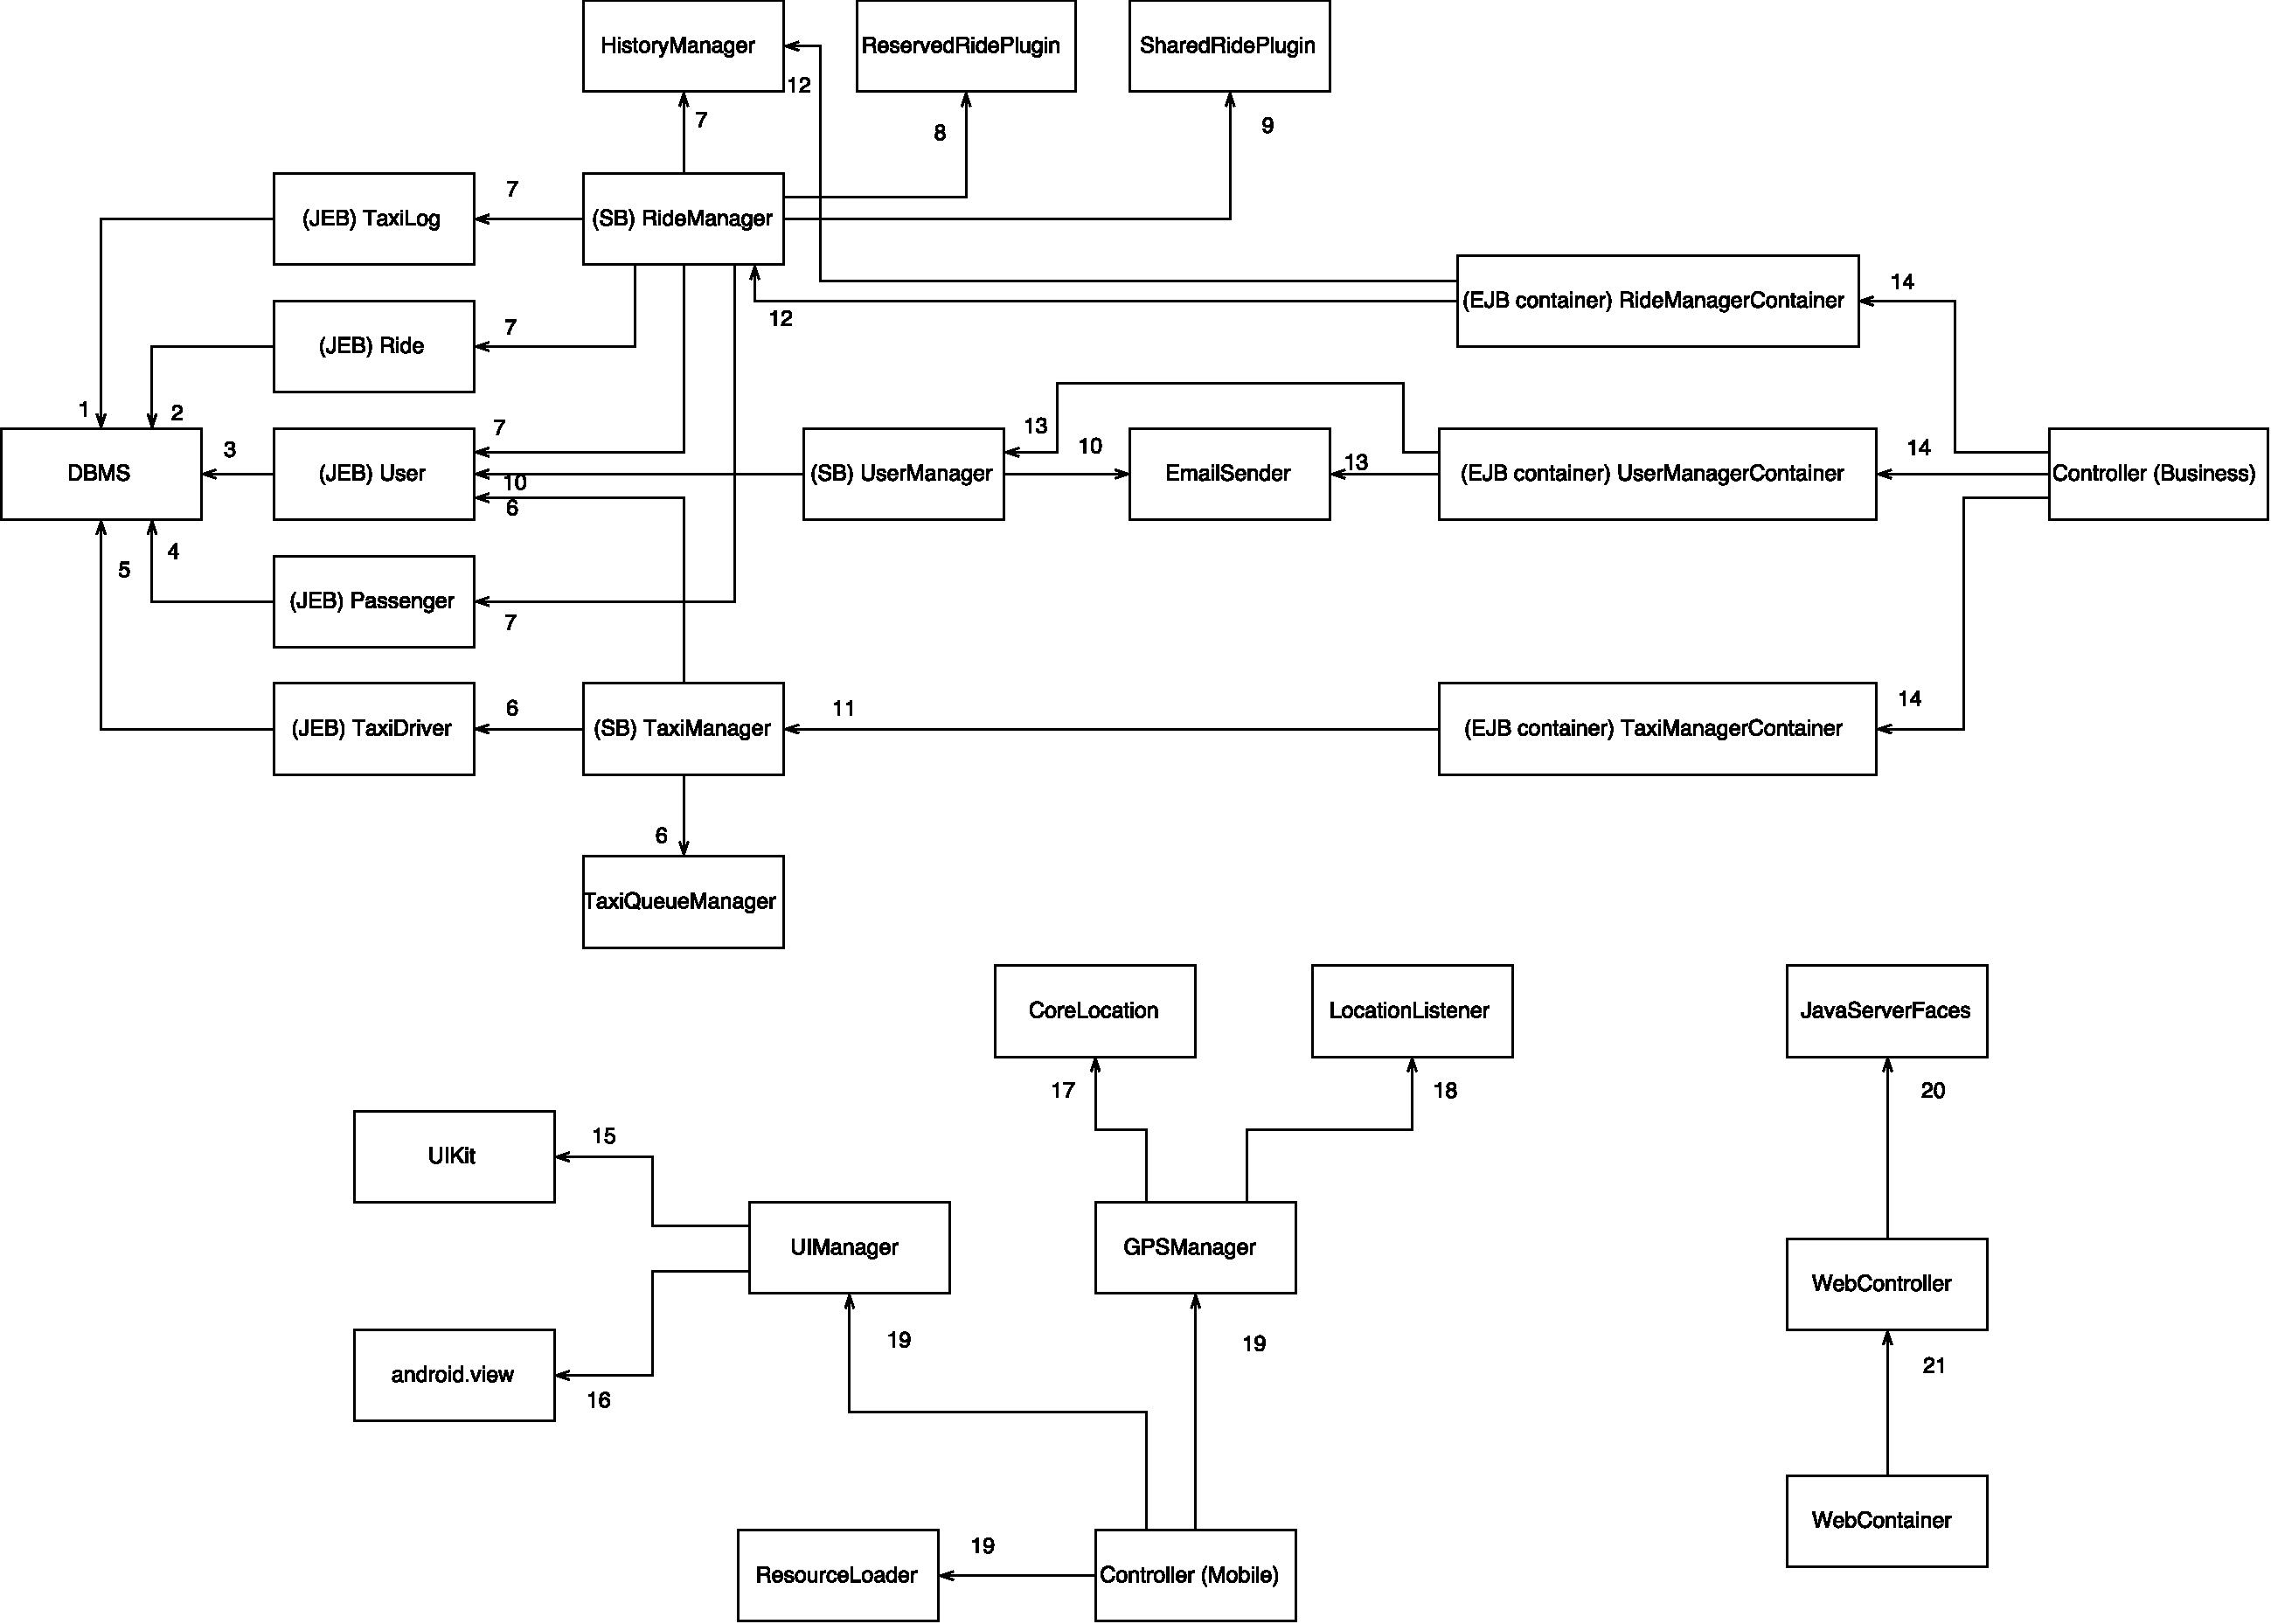
\includegraphics[width=\textwidth]{figures/components_integration.pdf}
    \caption{Diagram of the components integration.}
    \label{fig:components-integration}
\end{figure}
	

\subsection{Subsystem Integration Sequence}
The integration sequence of the subsystems is described in~\autoref{tab:subsystem-integration} and in~\autoref{fig:subsystem-integration}.

A choice was made to proceed with the integration process from the server side towards the client applications, integrating the mobile app before the web tier.
The reason to do so is that in order to have a functioning client you need to have a working business tier.
The business tier, instead, can be tested without any client, by making API calls also in an automated fashion.

By integrating the mobile application before the web tier, we aim to obtain a fully operational client-server system as soon as possible, since taxi drivers can't work without the mobile app.
The web tier is less essential and can be integrated after the app.

\begin{table}
    \centering
    \begin{tabular}{| l | l | l |}
        \hline
        N. & Subsystem & Integrates with \\
        \hline
        1 & Business tier & Database tier\\
        2 & Mobile application & Business tier\\
        3 & Web tier & Business tier\\
        4 & Client browser & Web tier\\
        \hline
    \end{tabular}
    \caption{Integration order of the subsystems described in~\autoref{sec:elements}.}
    \label{tab:subsystem-integration}
\end{table}

\begin{figure}[h]
    \centering
    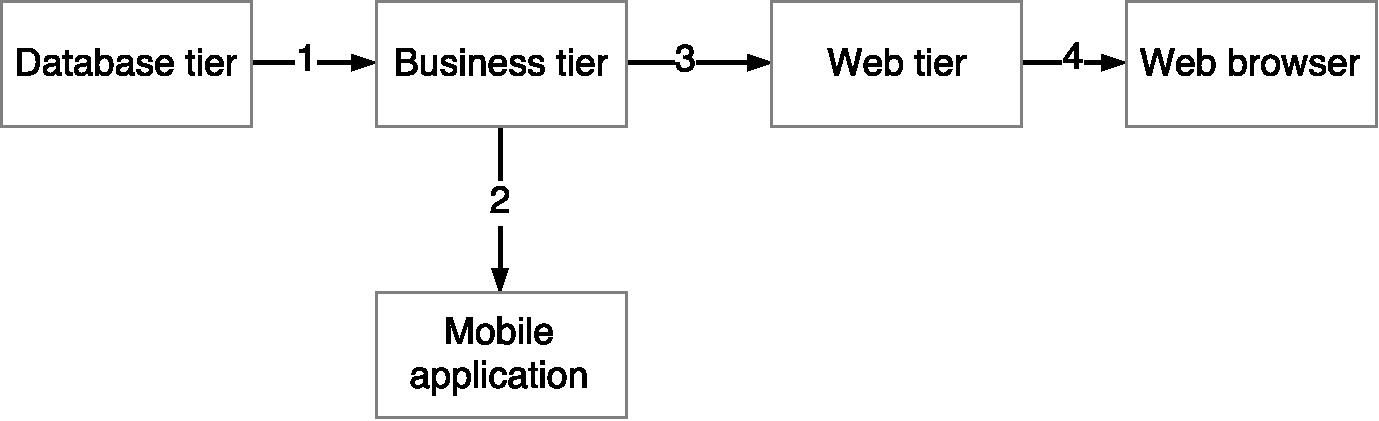
\includegraphics[width=\textwidth]{figures/subsystems_integration_dag.pdf}
    \caption{Directed Acyclic Graph representing the order of integration of the subsystems. See~\autoref{tab:subsystem-integration}.}
    \label{fig:subsystem-integration}
\end{figure}
